\subsection{能量量子化}
\textbf{黑体辐射}
\begin{tabularx}{\columnwidth}{XX}
  能量子关系 & $E=h\nu$ \\
  光子频率与波长 & $\nu=\frac{c}{\lambda}$ \\
  光子能量表达式 & $E=\frac{hc}{\lambda}$ \\
  振子能量量子化 & $E_n=nh\nu\quad(n=0,1,2,\cdots)$ \\
  峰值波长规律 & $\lambda_m T=\text{常量}$ \\
  黑体辐射规律（定性） & 温度越高，总辐射越强，峰值波长越短 \\
\end{tabularx}

\begin{center}
  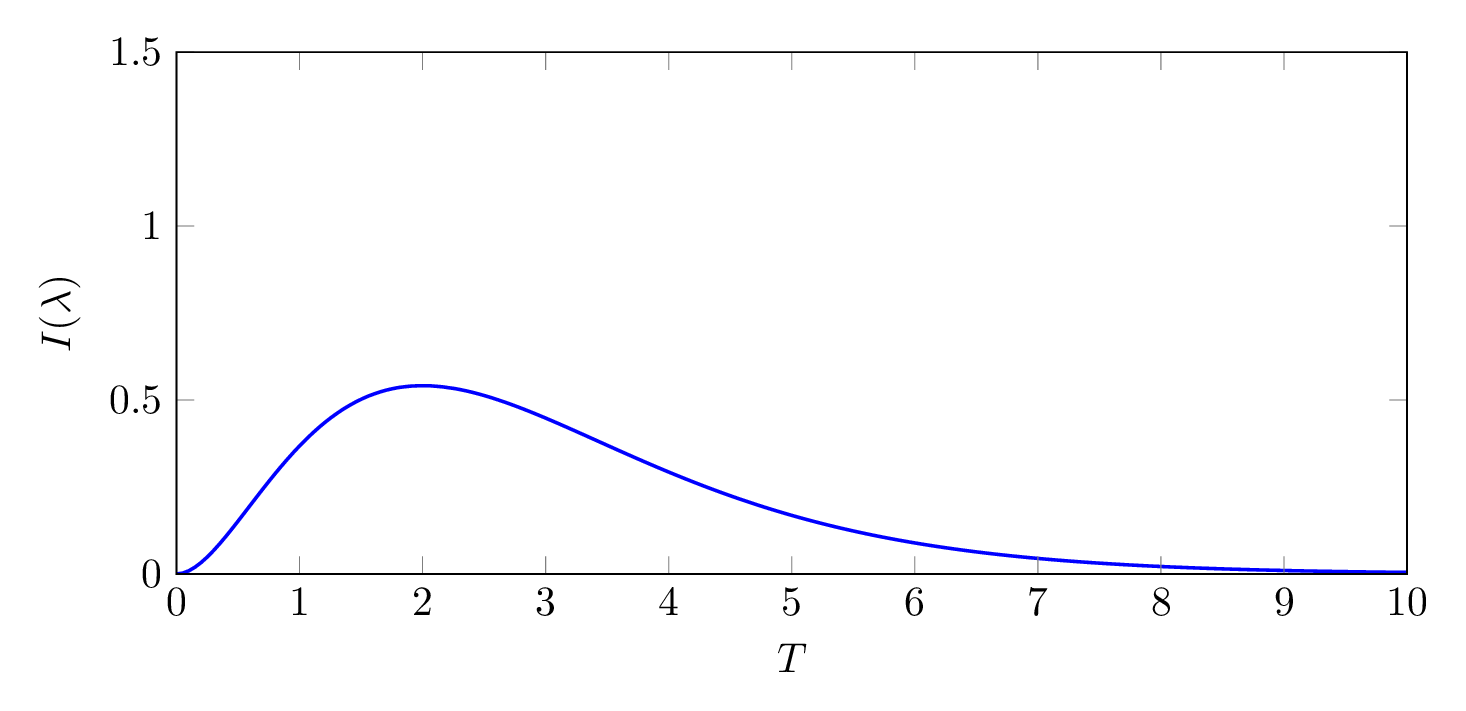
\includegraphics[width=0.72\columnwidth]{../assets/modern_blackbody_radiation.png}

  \vspace{4pt}
  {\small 黑体辐射强度随波长变化示意}
\end{center}

\begin{formulanotebox}
\begin{itemize}[leftmargin=1.5em]
  \item 黑体辐射图像判定中，高温曲线通常“更高且峰值左移”，低温曲线“更低且峰值右移”。
  \item $E=h\nu$ 描述单个能量子的能量；题目若给光强，还需结合单位时间光子数判断总能量。
\end{itemize}
\end{formulanotebox}

\begin{keypointbox}
\begin{itemize}[leftmargin=1.5em]
  \item 经典理论无法解释黑体辐射的短波异常，普朗克提出能量量子化假设。
  \item 量子化思想的核心是“能量交换不是连续取值，而是按能量子份额进行”，这是后续光电效应与波粒二象性的理论基础。
  \item 单个光子的能量由频率决定，频率越高能量越大；光强反映单位时间、单位面积内总能量大小。
\end{itemize}
\end{keypointbox}

\begin{casetypebox}[title={\strut\textcolor{white}{\bfseries 常见题型：黑体辐射图像判定}}]
\begin{itemize}[leftmargin=1.5em]
  \item 比较温度时看峰值位置和曲线整体高度：温度越高，峰值波长越短，曲线整体辐射强度越大。
  \item 图像横轴若为波长，高温曲线峰值向短波方向移动；横轴若为频率，高温峰值向高频方向移动。
  \item 不能只看某一波长处强度大小判断总辐射强弱，总辐射强度对应曲线下方面积。
\end{itemize}
\end{casetypebox}

\begin{casetypebox}[title={\strut\textcolor{white}{\bfseries 常见题型：能量量子化计算}}]
\begin{itemize}[leftmargin=1.5em]
  \item 已知频率用 $E=h\nu$，已知波长先用 $\nu=\frac{c}{\lambda}$，或直接用 $E=\frac{hc}{\lambda}$。
  \item $N$ 个相同频率光子的总能量为 $E_{\text{总}}=Nh\nu$；若已知总能量，可由 $N=\frac{E_{\text{总}}}{h\nu}$ 求光子数。
  \item 频率越大、波长越短，单个光子能量越大；不要把“光强更大”误判为“单个光子能量更大”。
\end{itemize}
\end{casetypebox}
